% PGFPlots ECDF calculated from the saved graph-evaluation JSON, 19 October 2026.
% First pass: 136 observations; first occurrence of each of 28 graph keys.
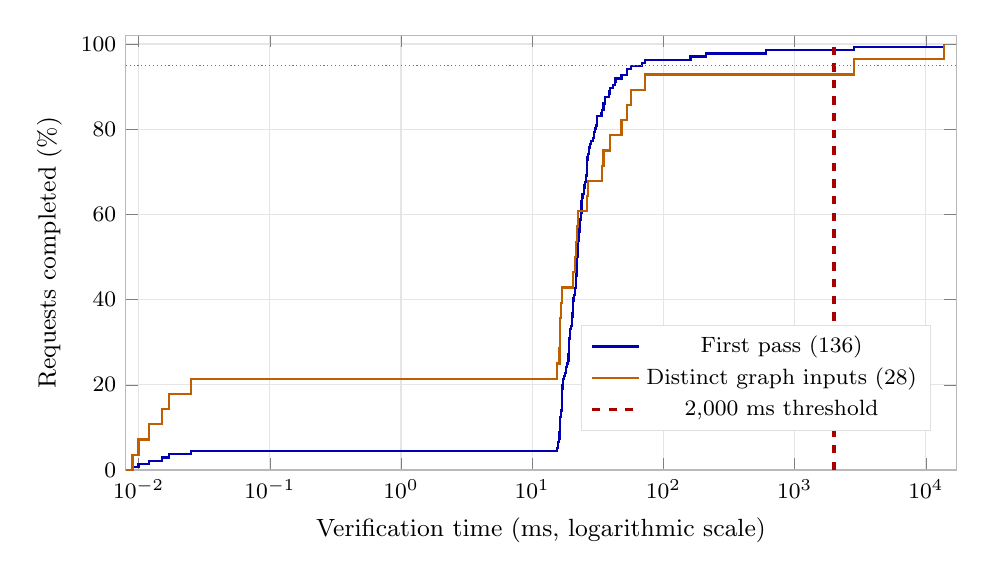
\begin{tikzpicture}
\begin{axis}[
    width=\linewidth,
    height=7.1cm,
    xmode=log,
    xmin=0.008, xmax=17000,
    ymin=0, ymax=102,
    xlabel={Verification time (ms, logarithmic scale)},
    ylabel={Requests completed (\%)},
    log basis x=10,
    xtick={0.01,0.1,1,10,100,1000,10000},
    xticklabels={$10^{-2}$,$10^{-1}$,$10^{0}$,$10^{1}$,$10^{2}$,$10^{3}$,$10^{4}$},
    ytick={0,20,40,60,80,100},
    grid=major,
    grid style={gray!20},
    tick label style={font=\footnotesize},
    label style={font=\small},
    legend style={font=\footnotesize,draw=gray!25,fill=white,at={(0.97,0.09)},anchor=south east},
    axis line style={gray!55},
    clip=true
]
\addplot+[const plot,mark=none,thick,color=blue!70!black] coordinates {
    (0.008,0)
    (0.0090,0.73529)
    (0.0100,1.47059)
    (0.0120,2.20588)
    (0.0150,2.94118)
    (0.0170,3.67647)
    (0.0250,4.41176)
    (15.5180,5.14706)
    (15.6410,5.88235)
    (15.7770,6.61765)
    (15.9380,7.35294)
    (16.1270,8.08824)
    (16.1290,8.82353)
    (16.2080,9.55882)
    (16.3340,10.29412)
    (16.3400,11.02941)
    (16.3550,11.76471)
    (16.3820,12.50000)
    (16.5130,13.23529)
    (16.6490,13.97059)
    (16.7600,14.70588)
    (16.7630,15.44118)
    (16.8200,16.17647)
    (16.8830,16.91176)
    (16.8890,17.64706)
    (16.9380,18.38235)
    (16.9630,19.11765)
    (17.0050,19.85294)
    (17.1320,20.58824)
    (17.2240,21.32353)
    (17.3960,22.05882)
    (17.8620,22.79412)
    (18.0470,23.52941)
    (18.2080,24.26471)
    (18.4260,25.00000)
    (18.8410,25.73529)
    (18.8830,26.47059)
    (18.9260,27.20588)
    (18.9670,27.94118)
    (18.9810,28.67647)
    (19.0310,29.41176)
    (19.0770,30.14706)
    (19.1600,30.88235)
    (19.3840,31.61765)
    (19.4380,32.35294)
    (19.4970,33.08824)
    (19.8730,33.82353)
    (19.9760,34.55882)
    (19.9810,35.29412)
    (20.1070,36.02941)
    (20.2540,36.76471)
    (20.3930,37.50000)
    (20.4820,38.23529)
    (20.5280,38.97059)
    (20.5870,39.70588)
    (20.6140,40.44118)
    (20.9020,41.17647)
    (21.1650,41.91176)
    (21.2440,42.64706)
    (21.5430,43.38235)
    (21.5730,44.11765)
    (21.6240,44.85294)
    (21.7040,45.58824)
    (21.7730,46.32353)
    (21.8530,47.05882)
    (21.8580,47.79412)
    (22.0050,48.52941)
    (22.0210,49.26471)
    (22.0450,50.00000)
    (22.1940,50.73529)
    (22.2020,51.47059)
    (22.2990,52.20588)
    (22.4200,52.94118)
    (22.4270,53.67647)
    (22.5450,54.41176)
    (22.5770,55.14706)
    (22.8210,55.88235)
    (22.9460,56.61765)
    (22.9640,57.35294)
    (23.1680,58.08824)
    (23.2790,58.82353)
    (23.3940,59.55882)
    (23.4450,60.29412)
    (23.7100,61.02941)
    (23.7480,61.76471)
    (23.7700,62.50000)
    (23.7820,63.23529)
    (24.1060,63.97059)
    (24.1760,64.70588)
    (24.6960,65.44118)
    (24.9350,66.17647)
    (25.0460,66.91176)
    (25.3440,67.64706)
    (25.5270,68.38235)
    (25.7450,69.11765)
    (26.0000,69.85294)
    (26.0310,70.58824)
    (26.2360,71.32353)
    (26.2420,72.05882)
    (26.2730,72.79412)
    (26.3390,73.52941)
    (26.5040,74.26471)
    (26.9290,75.00000)
    (26.9970,75.73529)
    (27.4750,76.47059)
    (27.8820,77.20588)
    (28.9600,77.94118)
    (29.3710,78.67647)
    (29.5070,79.41176)
    (29.9270,80.14706)
    (30.8030,80.88235)
    (31.0160,81.61765)
    (31.2490,82.35294)
    (31.3040,83.08824)
    (33.7010,83.82353)
    (33.8460,84.55882)
    (34.9240,85.29412)
    (34.9370,86.02941)
    (35.6280,86.76471)
    (35.9150,87.50000)
    (38.4330,88.23529)
    (38.7370,88.97059)
    (39.1160,89.70588)
    (41.2990,90.44118)
    (42.9050,91.17647)
    (43.0430,91.91176)
    (47.9180,92.64706)
    (52.4810,93.38235)
    (53.0190,94.11765)
    (56.6020,94.85294)
    (68.4440,95.58824)
    (71.9540,96.32353)
    (160.5490,97.05882)
    (211.0120,97.79412)
    (607.4290,98.52941)
    (2846.4390,99.26471)
    (13662.3040,100.00000)
};
\addlegendentry{First pass (136)}
\addplot+[const plot,mark=none,thick,color=orange!75!black] coordinates {
    (0.008,0)
    (0.0090,3.57143)
    (0.0100,7.14286)
    (0.0120,10.71429)
    (0.0150,14.28571)
    (0.0170,17.85714)
    (0.0250,21.42857)
    (15.5180,25.00000)
    (16.1290,28.57143)
    (16.3400,32.14286)
    (16.3820,35.71429)
    (16.6490,39.28571)
    (16.8830,42.85714)
    (20.4820,46.42857)
    (21.1650,50.00000)
    (21.7040,53.57143)
    (21.8530,57.14286)
    (22.1940,60.71429)
    (26.2360,64.28571)
    (26.5040,67.85714)
    (33.8460,71.42857)
    (34.9370,75.00000)
    (39.1160,78.57143)
    (47.9180,82.14286)
    (52.4810,85.71429)
    (56.6020,89.28571)
    (71.9540,92.85714)
    (2846.4390,96.42857)
    (13662.3040,100.00000)
};
\addlegendentry{Distinct graph inputs (28)}
\addplot+[mark=none,very thick,dashed,color=red!65!black]
    coordinates {(2000,0) (2000,100)};
\addlegendentry{2,000 ms threshold}
\addplot+[mark=none,densely dotted,thin,color=black!55,forget plot]
    coordinates {(0.008,95) (17000,95)};
\end{axis}
\end{tikzpicture}
